\section{如何开始}
{\BIThesis} 为各位在北京理工大学就读的本科同学提供了基于北京理工大学计算机学院教务部给出的“北京理工大学计算机学院本科生毕业论文:开题报告”与北京理工大学教务部提供的“北京理工大学本科生毕业设计:论文模板(目前是 2019 届版本)”的 \LaTeX 样版。借助于 {\BIThesis} 的 \LaTeX 模板,你可以在保证论文格式整齐、完美、符合要求的前提下,专注于学术研究、项目实现,从而顺利完成你的学术项目。

本“使用手册”希望为大家全面的介绍 {\LaTeX} 环境的搭建方法、{\BIThesis} 的使用方法,从而快速掌握使用 {\LaTeX} 排版引擎进行基本的论文撰写的方法,完成符合学校要求的学位论文。{\BIThesis} 目前使用 GitHub 进行维护,官方项目地址位于:

\begin{center}
\color{ForestGreen}\href{https://github.com/spencerwooo/BIThesis}{\texttt{https://github.com/spencerwooo/BIThesis}}
\end{center}

\subsection{在线说明文档:Wiki}
和本手册的目标类似,{\BIThesis} 项目同样维护了一个在线版本的说明文档,位于:{\href{https://github.com/spencerwooo/BIThesis/wiki}{BIThesis - wiki}},二者的目的、内容、功能类似,且会随着模板的开发与维护同步更新。

{\BIThesis} 在线说明文档目前拥有与本手册一致的如下模块:

\begin{enumerate}
\item \href{https://github.com/spencerwooo/BIThesis/wiki}{主页:Home}
\item \href{https://github.com/spencerwooo/BIThesis/wiki/First-things-first}{如何开始:First things first }
\item \href{https://github.com/spencerwooo/BIThesis/wiki/Using-one-of-the-templates}{使用其中一个模板:Using one of the templates}
\item \href{https://github.com/spencerwooo/BIThesis/wiki/Proposal-Report}{本科生开题报告:Proposal report}
\item \href{https://github.com/spencerwooo/BIThesis/wiki/Final-Graduation-Thesis}{本科生毕业论文:Graduation thesis}
\item \href{https://github.com/spencerwooo/BIThesis/wiki/Lab-Report}{本科生实验报告:Lab report}
\item \href{https://github.com/spencerwooo/BIThesis/wiki/Converting-to-Word}{将 LaTeX 文档转换为 Word:Converting to Word}
\end{enumerate}

接下来,我们正式开始介绍 {\LaTeX} 与 {\BIThesis} 的使用方法。

\subsection{准备工作}
首先,在使用模板之前,你需要在本机安装 \LaTeX 环境。一个完整的 \LaTeX 环境包括:

\begin{itemize}
  \item 开源免费的 \LaTeX 发行版(包含有必备的 \LaTeX 编译器与有用的宏包),与……
  \item 一个得心应手的 \LaTeX 编辑器
\end{itemize}

我们在 Windows、macOS 与 Linux 环境中均可以使用 \LaTeX 进行文档撰写。按照操作系统的不同,我们分别进行介绍。

\subsection{下载合适的 \LaTeX 发行版}
\importantbox{\textbf{注意:}{\BIThesis} 中参考文献为了和校方规定的模板格式《信息与文献参考文献著录规则》(\href{http://openstd.samr.gov.cn/bzgk/gb/newGbInfo?hcno=7FA63E9BBA56E60471AEDAEBDE44B14C}{GB/T 7714—2015})保持一致,使用了仅支持 \TeX Live 2019 版本的宏包,如果你曾经安装过 \TeX Live 且目前正在使用的 \TeX Live 版本不是 2019 版本,那么请及时更新为最新的 \TeX Live 2019 版本。}

\subsubsection{Windows 和 Linux 系统}
对于 Windows 和 Linux 系统,我们可以直接下载使用 \href{https://www.tug.org/texlive/}{\TeX Live 发行版}。

\paragraph{在线安装} 官方的安装指南位于:\href{https://www.tug.org/texlive/acquire-netinstall.html}{Installing \TeX Live over the Internet}。使用这一方法会下载 \texttt{install-tl-windows.exe}(Windows)或 \texttt{install-tl-unx.tar.gz}(Linux),之后运行相应的可执行程序,安装程序即可将整个 \TeX Live 发行版下载安装到我们本机。(通常会安装 3GB 左右的程序。)

\begin{figure}[H]
  \centering
  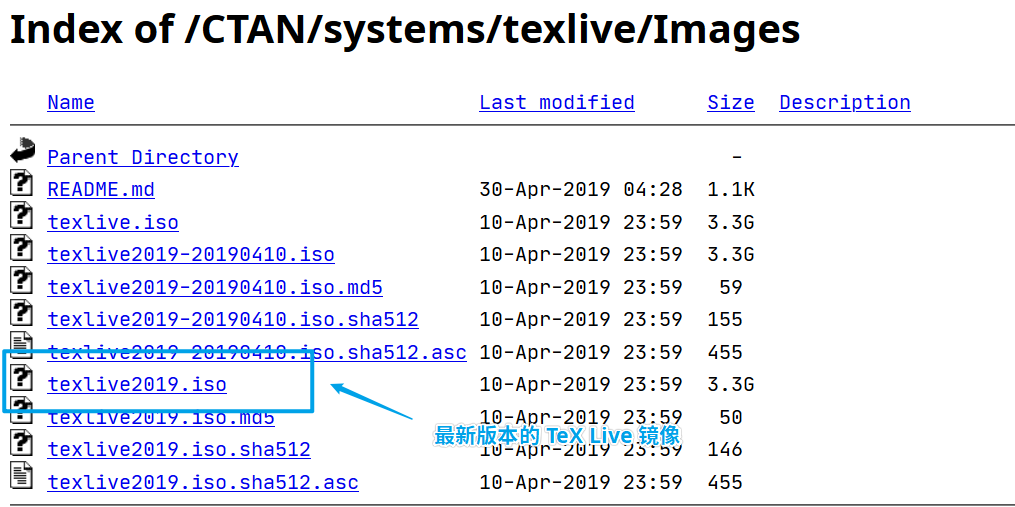
\includegraphics[width=\textwidth]{images/bit_mirror_texlive.png}
  \caption{北京理工大学开源镜像站 \TeX Live 下载}
  \label{mirrorbit}
\end{figure}

\paragraph{离线安装} 使用北京理工大学校园网的同学也可以直接使用我校官方 \TeX Live 镜像进行安装。我校 \TeX Live 镜像资源位于 \href{https://mirrors.bit.edu.cn/CTAN/systems/texlive/Images}{/CTAN/systems/texlive/Images},其中我们选择下载 \texttt{texlive2019.iso} 即可,如图 \ref{mirrorbit} 所示。Windows 10 可直接挂载 ISO 镜像(双击即可),其余系统用合适的软件也可。之后在打开的文件夹中点击执行 \texttt{install-tl-windows}(Windows)或 \texttt{install-tl}(Linux)即可离线安装全部 \TeX Live 组件。

\paragraph{使用包管理工具进行安装} 使用 Linux 系统的同学也可以选择使用合适的包管理工具进行 \TeX Live 的安装。以 Ubuntu 为例子,只需要运行下面命令,即可下载安装整个 \TeX Live 发行版。

\begin{minted}[
  frame=single
]{bash}
sudo apt install texlive
\end{minted}

\subsubsection{macOS 系统}
对于 macOS 系统,我们可以直接下载使用 \href{https://www.tug.org/mactex/}{Mac\TeX 发行版}。Mac\TeX 发行版是以 pkg 文件进行发布安装的,我们进入 \href{https://www.tug.org/mactex/mactex-download.html}{Max\TeX 的下载页面},点击下载 \texttt{MacTeX.pkg} 即可下载完整的 Mac\TeX 安装包(大约 3.9GB)。之后双击运行即可安装。

另外,使用 Homebrew 包管理的同学,也可以通过 Homebrew Cask 直接安装 Mac\TeX:

\begin{minted}[
  frame=single
]{bash}
# 加载 Homebrew Cask
brew tap caskroom/cask

# 利用 Cask 安装 MacTeX
brew cask install mactex
\end{minted}

\subsubsection{确认安装}
为了保证我们 \LaTeX 发行版的安装没有问题,我们需要验证一下 \LaTeX 编译工具的安装情况。我们打开终端(Windows 打开 PowerShell、macOS 打开 Terminal、Linux 打开你所使用的终端模拟器),在其中输入下面的命令:

\begin{itemize}
  \item 验证 \texttt{xelatex} {\LaTeX} 编译器的安装情况:
  \begin{minted}[
    frame=single
  ]{bash}
  xelatex --version
  \end{minted}
  \begin{figure}[H]
    \flushright
    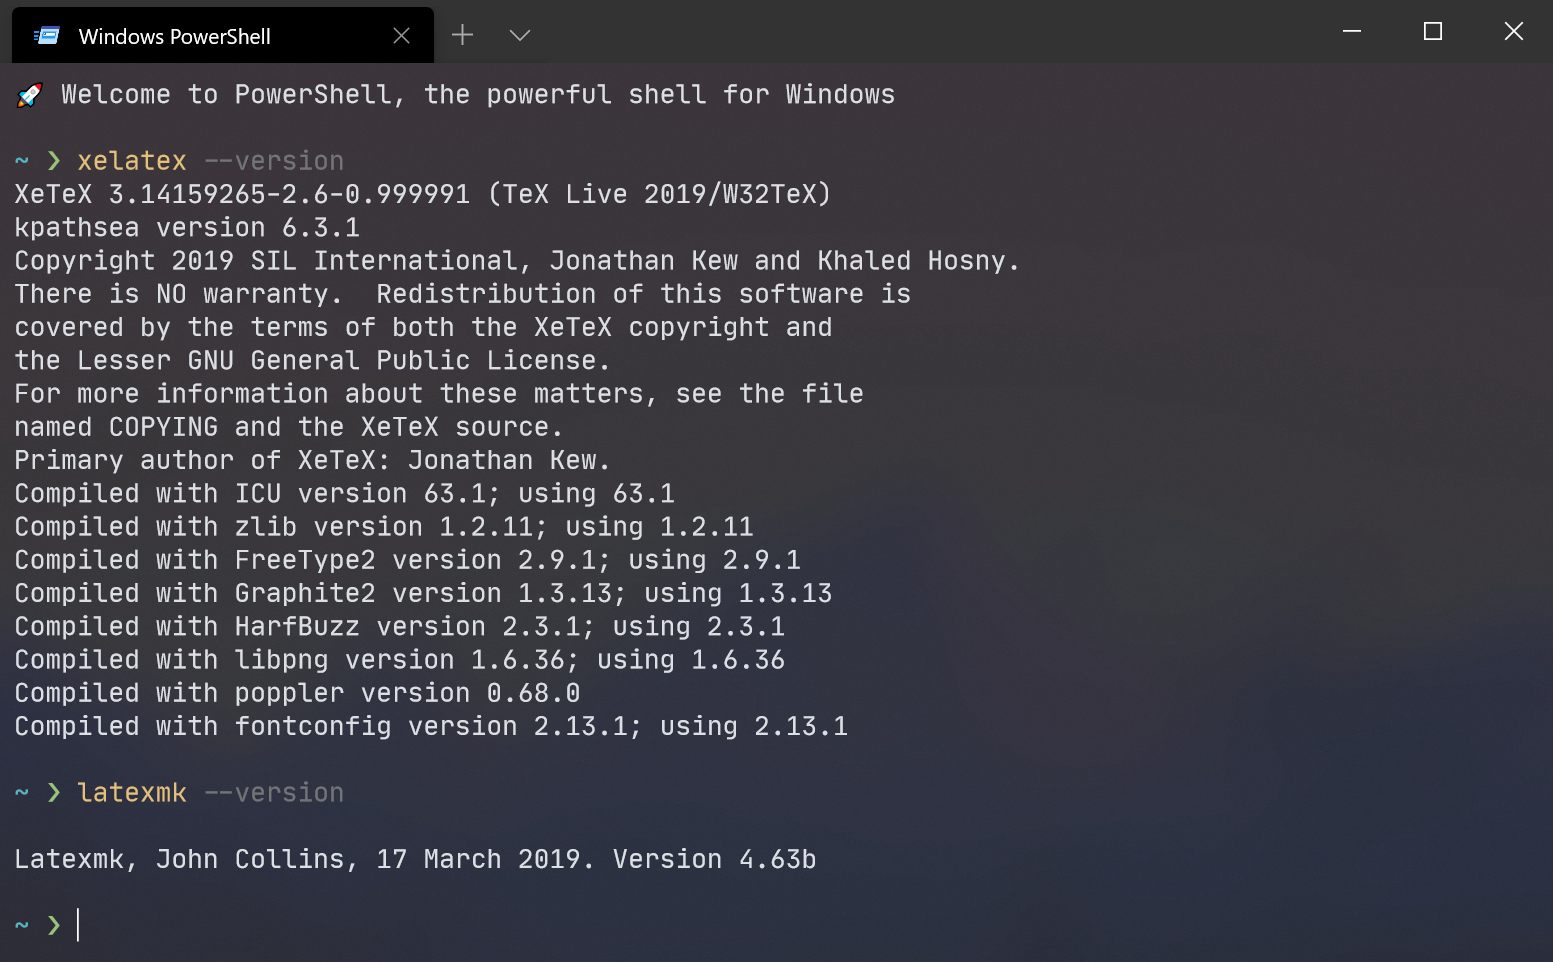
\includegraphics[width=0.93\textwidth]{images/xelatex.png}
    \caption{\hologo{XeLaTeX} 安装成功输出}
    \label{xelatex}
  \end{figure}
  \item 验证 \texttt{biber} 参考文献编译器的安装情况:
  \begin{minted}[
    frame=single
  ]{bash}
  biber --version
  \end{minted}
  \begin{figure}[H]
    \flushright
    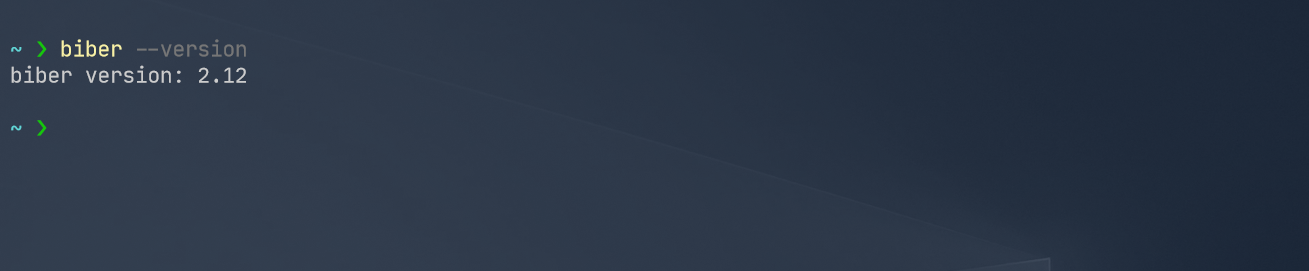
\includegraphics[width=0.93\textwidth]{images/biber.png}
    \caption{\hologo{biber} 安装成功输出}
    \label{biber}
  \end{figure}
\end{itemize}

出现如图 \ref{xelatex} 与 \ref{biber} 类似的输出,说明我们编译器安装应该是没有问题的。

\subsection{挑选合适的 \LaTeX 编辑器}
理论上来说,任何一个“文本编辑器”均可以用来撰写 {\LaTeX} 文档,但是一个得心应手的 {\LaTeX} 编辑器一定会让我们撰写论文的效率大增。

\subsubsection{使用 VS Code 配合 {\LaTeX} Workshop 插件编辑 \LaTeX 文档}
VS Code 是微软开发的基于 Electron 跨平台技术的新晋代码编辑器,开源免费、拓展性强、功能强大,是当代开发者的首选。用 VS Code 配合 {\LaTeX} Workshop 插件我们可以打造一个强大的 {\LaTeX} 编辑器。

\begin{figure}[H]
  \centering
  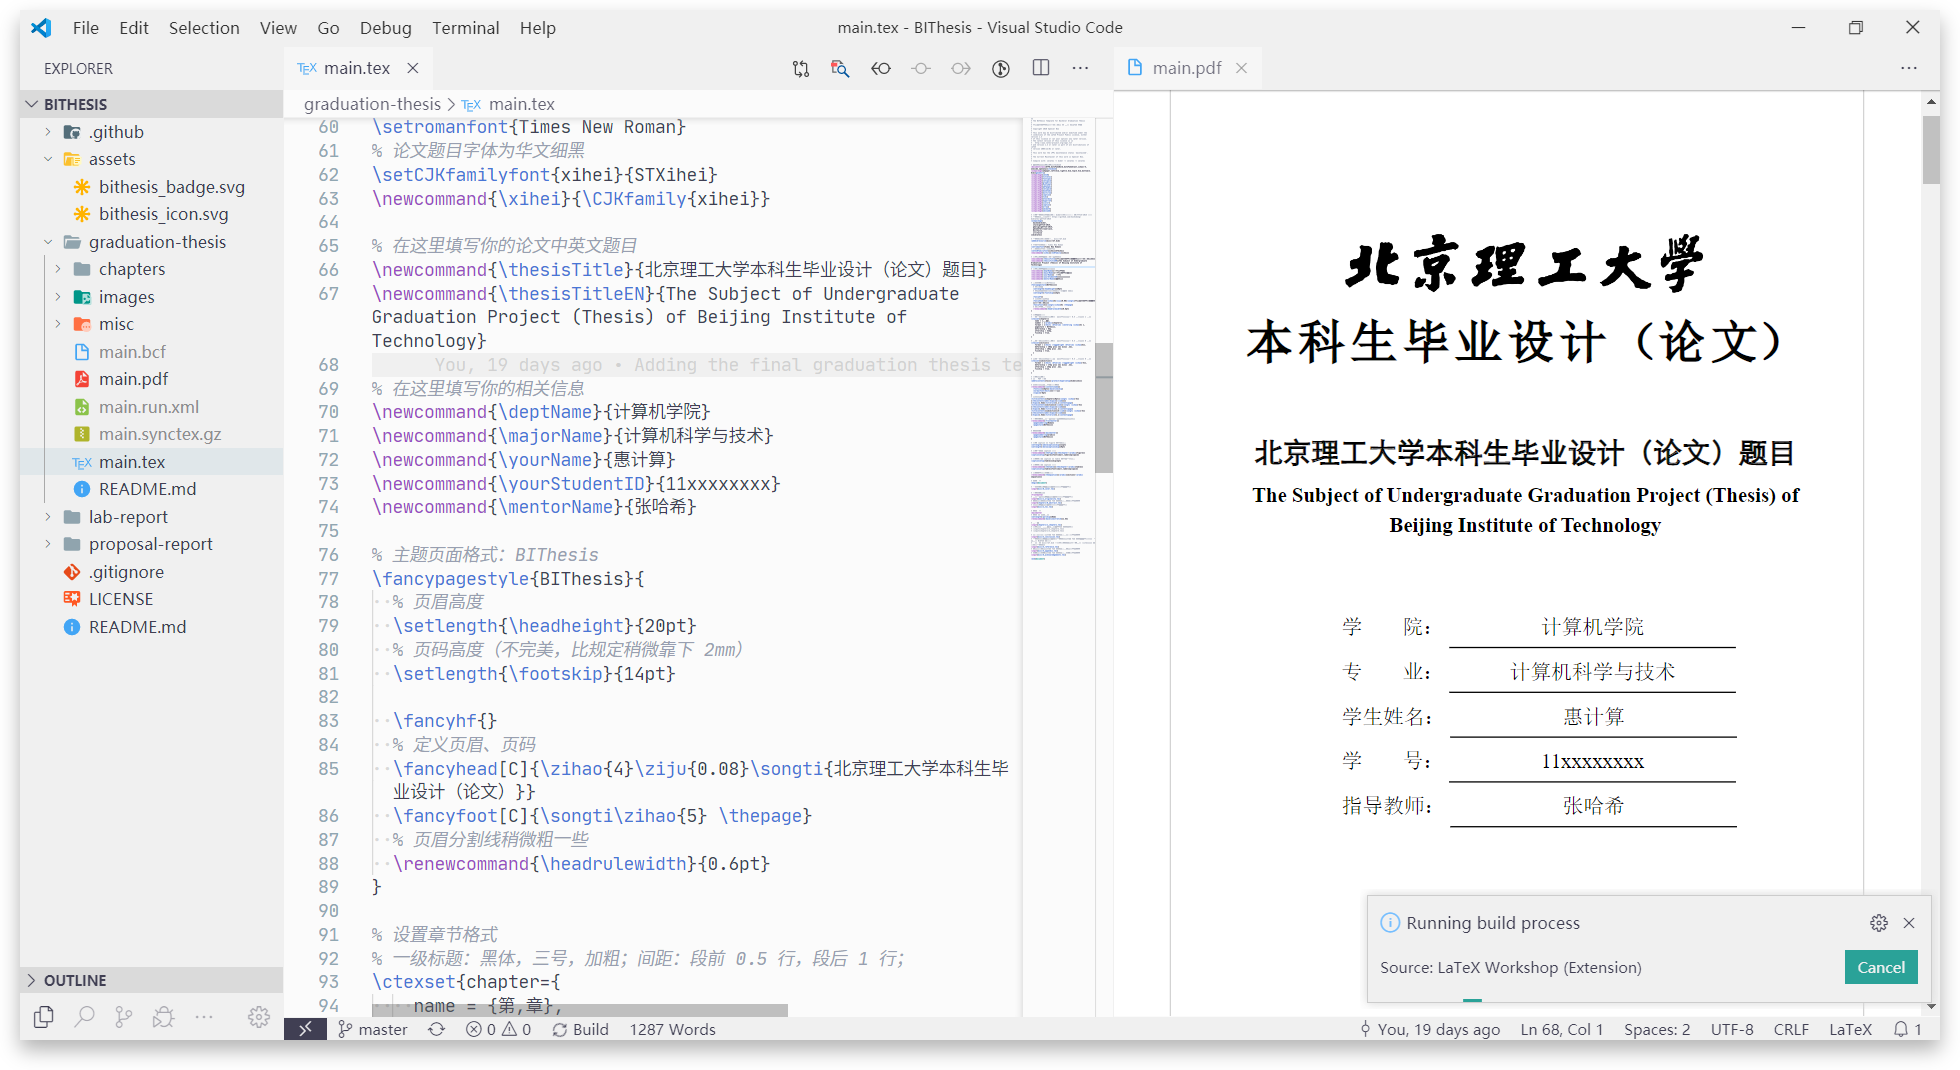
\includegraphics[width=\textwidth]{images/vscode.png}
  \caption{VS Code 代码编辑器}
\end{figure}

\begin{itemize}
  \item 安装 VS Code 编辑器:\href{https://code.visualstudio.com/}{Visual Studio Code - Code editing. Redefined.}
  \item 安装插件:
  \begin{itemize}
    \item 安装 {\LaTeX} Workshop 插件:\href{https://marketplace.visualstudio.com/items?itemName=James-Yu.latex-workshop}{Visual Studio Code LaTeX Workshop Extension}
    \begin{itemize}
      \item 提供基本的浏览、编辑、自动补全、自动格式化 {\LaTeX} 文档的功能
      \item 提供在 VS Code 内直接预览 {\LaTeX} 文档编译得到的 PDF 的功能
      \item 提供编译工具链、自定义编译方法等功能
      提供 SyncTeX 双向定位功能({\LaTeX} 源码 $\longleftrightarrow$ PDF)

    \end{itemize}
    \item (可选)安装 {\LaTeX} Utilities 插件:\href{https://marketplace.visualstudio.com/items?itemName=tecosaur.latex-utilities}{Visual Studio Code LaTeX Utilities}
    \begin{itemize}
      \item 提供实时 {\LaTeX} 文档字数统计的功能
      \item 提供与参考文献管理工具 Zotero 连接的功能
    \end{itemize}
  \end{itemize}
\end{itemize}

使用 VS Code 作为 {\LaTeX} 编辑器时,我们需要特别配置编译工具 \texttt{tools} 与编译工具链 \texttt{recipes}。对于包含有目录、参考文献、图片与表格引用的 {\LaTeX} 文档,我们往往需要使用多个编译工具串联编译,VS Code 就是在这里定义我们编译所使用的工具。

VS Code 的设置项目可以通过快捷键 \keys{\ctrl + ,}(macOS \keys{\cmd + ,})打开 UI 设置界面,之后点击右上角 \texttt{Open Settings (JSON)} 按钮即可打开相应的 JSON 格式配置文件,我们在这里即可定义 {\LaTeX} 编译工具。其中:

\begin{itemize}
  \item “编译工具”是在 \texttt{"latex-workshop.latex.tools": [ ... ]} 处进行定义,比如我们定义使用 \texttt{latexmk} 编译,即可在这里声明:
  \begin{minted}[
  frame=single
  ]{json}
  "latex-workshop.latex.tools": [
    {
      "name": "latexmk",
      "command": "latexmk",
      "args": [
        "-synctex=1",
        "-interaction=nonstopmode",
        "-file-line-error",
        "-pdf",
        "-outdir=%OUTDIR%",
        "-cd",
        "%DOC%"
      ],
      "env": {}
    }
  ]
  \end{minted}
  \item “编译工具链”是在 \texttt{"latex-workshop.latex.recipes": [ ... ]} 处进行定义,比如我们为了正确生成目录,需要调用两次 \texttt{xelatex},那么我们即可这样定义:
  \begin{minted}[
  frame=single
  ]{json}
  "latex-workshop.latex.recipes": [
    {
      "name": "xelatex * 2",
      "tools": [
          "xelatex",
          "xelatex"
      ]
    }
  ]
  \end{minted}
\end{itemize}

有关编译命令与编译工具链的更多配置,请参考每一种模板的编译方法,具体问题、具体分析。

\subsubsection{使用 \TeX studio 编辑 \LaTeX 文档}
\TeX studio 是老牌 {\LaTeX} 编辑器,使用跨平台技术 Qt 编写而成。虽然界面相对老旧,但是依旧可靠。我们可以去 \href{https://www.texstudio.org/}{\TeX studio 的官网}下载安装各个系统版本的 \TeX studio。

\begin{figure}[H]
  \centering
  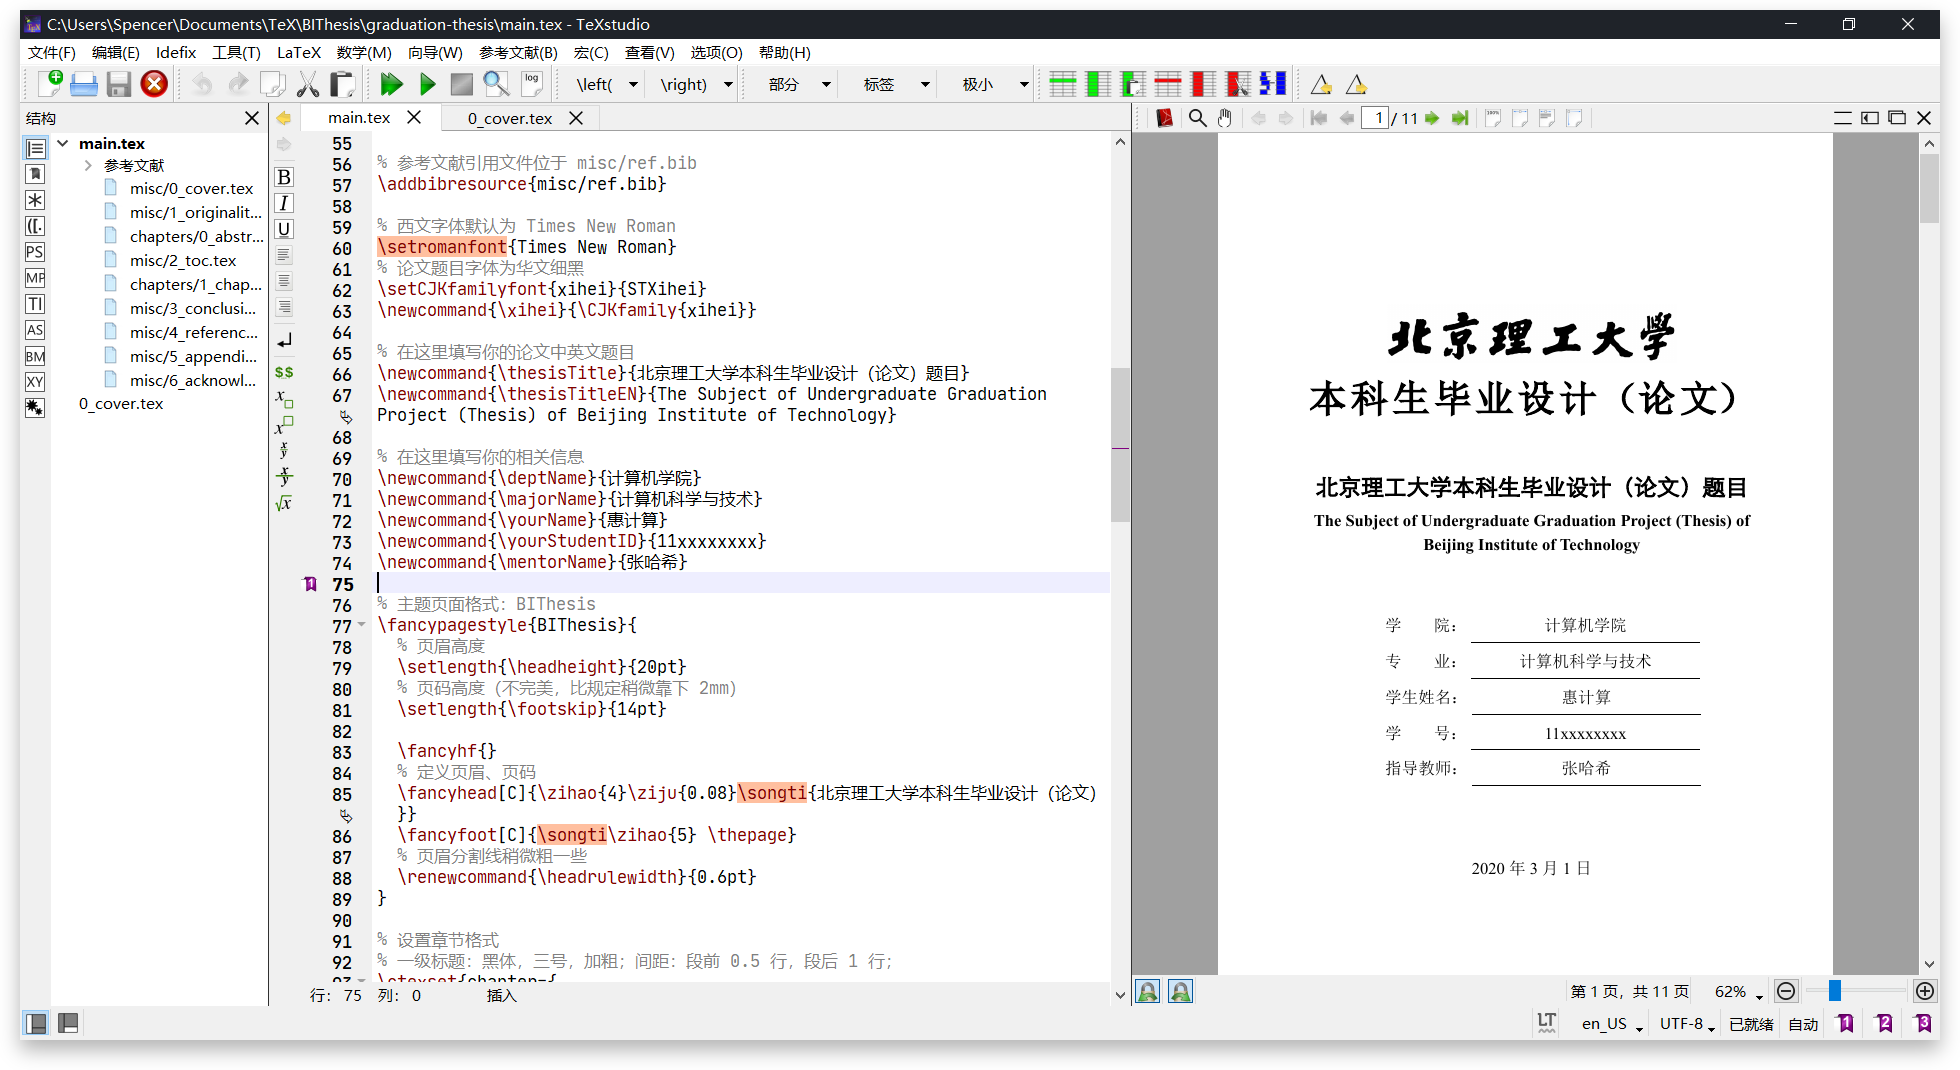
\includegraphics[width=\textwidth]{images/texstudio.png}
  \caption{\TeX studio 老牌 {\LaTeX} 编辑器}
\end{figure}

默认情况下 \TeX studio 的编译工具链均已经配置完毕,基本开箱即用。我们只需要在 \TeX studio 的设置中定义编译所用的编译器即可。

\subsubsection{徒手编译}

当然,你完全可以不借助任何编辑器,直接使用“命令行”编译 {\LaTeX} 文档。以我们模板中比较常见的四步走 \texttt{xelatex -> biber -> xelatex -> xelatex} 为例子,你可以用下面的命令编译主文档为 \texttt{main.tex} 的 {\LaTeX} 项目:

\begin{minted}[frame=single]{bash}
# 第一步 xelatex
xelatex -no-pdf --interaction=nonstopmode main
# 第二步 biber
biber main
# 第三步 xelatex
xelatex -no-pdf --interaction=nonstopmode main
# 第四步 xelatex
xelatex --interaction=nonstopmode main
\end{minted}

\tipbox{另外,如果你是特别不差钱的 Mac 用户,希望用最好用最牛逼的 {\LaTeX} 编辑器,你也可以去购买目前售价 \$29.99 美元(约合人民币 209.69 元)的 Texpad。使用 macOS、iOS 原生技术栈开发,Texpad 可能是目前使用体验最顺滑的 {\LaTeX} 编辑器,另外由于 Texpad 使用私有 {\LaTeX} 发行版,使得 Texpad 支持实时预览成果 PDF 与双向同步滚动支持。有这方面需要(与金钱)的同学可以考虑入手。}

准备就绪后,我们就可以开始使用 {\BIThesis} 提供的模板进行 {\LaTeX} 文档的撰写啦!
